% Define document class
\documentclass[twocolumn]{aastex631}
\usepackage{showyourwork}
\usepackage{CJK}

% Begin!
\begin{document}

% Title
\title{Global simulation of thermal torques}

% Author list
\author[0000-0002-6650-3829]{Sabina Sagynbayeva}
\affiliation{Department of Physics and Astronomy, Stony Brook University, Stony Brook, NY 11794, USA}

\author[0000-0002-2624-3399]{Yan-Fei Jiang(姜燕飞)}
\affiliation{Center for Computational Astrophysics, Flatiron Institute, 162 Fifth Avenue, New York, NY 10010, USA}

\author{Zhaohuan Zhu(朱照寰)}
\affiliation{Department of Physics and Astronomy, University of Nevada, Las Vegas, 4505 S.~Maryland Parkway, Las Vegas, NV~89154-4002, USA}

\author[0000-0001-5032-1396]{Philip J. Armitage}
\affiliation{Center for Computational Astrophysics, Flatiron Institute, 162 Fifth Avenue, New York, NY 10010, USA}
\affiliation{Department of Physics and Astronomy, Stony Brook University, Stony Brook, NY 11794, USA}

% Abstract with filler text
\begin{abstract}
   
\end{abstract}

% Main body with filler text
\section{Introduction} 
\label{sec:intro}
We follow up \citet{hankla20} :)

\section{Methods}
\label{sec:methods}

\subsection{Disk model}
Isentropic disk model from \citet{Fung_2017}.
The simulations are performed in spherical coordinates, where $r$, $\phi$, and $\theta$ denote the usual radial, azimuthal, and polar coordinates, respectively. 

\begin{equation}\label{eq:potential}
\begin{aligned}
     \Phi = & -\frac{G(M_*+M_p)}{1+q} \bigg[\frac{1}{r} \\
     & + \frac{q}{\sqrt{r^2+R_p^2-2rR_p\cos{\phi'}+\epsilon^2}} - \frac{qR\cos{\phi'}}{R_p^2}\bigg] \\
\end{aligned}
\end{equation}

In eq. \ref{eq:potential}, $q = M_p/M_*$ is the mass ratio of a protoplanet to a star, $\epsilon$ is the smoothing length of the planet's potential, and $\phi'= \phi-\phi_p$ denotes the azimuthal separation from the planet. $GM=1$, $R_p=1$.

Keplerian velocity $v_k=\sqrt{\frac{GM}{r}}$ and keplerian frequency $\Omega_k=\sqrt{\frac{GM}{r^3}}$ equal to 1 at the planet's orbit.

$v_p$ - planet's orbital speed. 
$q = 1.5\times 10^{-5} \approx 5 M_{\oplus}$

The planet is introduced to the disk gradually, where its mass increases to the desired value over the first orbit.

The simulation domain spans $0.65R_p$ to $1.35R_p$ in the radial, and the full $2\pi$ in azimuth.

The Hill radius of a planet is:
\begin{equation}\label{eq:Hill}
    r_H=R_p\left(\frac{q}{3}\right)^{\frac{1}{3}}
\end{equation}

$r_s$ is a small fraction of $r_H$, between 3\% to 10\% of $r_H$.

The isentropic equation of state:
\begin{equation}\label{eq:pressure}
    p = \frac{c_0^2\rho_0}{\gamma}\left(\frac{\rho}{\rho_0}\right)^\gamma
\end{equation}

In Eq. \ref{eq:pressure}, $c_0$ is the isothermal sound speed when $\rho=\rho_0=1$. 
The disk's scale height $H = 0.05$ scales the sound speed as $c_0 = H\Omega=0.05$.

\subsubsection{Initial conditions}
For hydrostatic equilibrium:
\begin{equation}\label{eq:density}
\begin{aligned}
     \rho = & \rho_0 \bigg[\left(\frac{R}{R_p}\right)^{(-\beta+\frac{3}{2})\frac{2(\gamma-1)}{\gamma+1}} \\ 
    & - \frac{GM(\gamma-1)}{c_0^2}\left(\frac{1}{R}-\frac{1}{r}\right)\bigg]^{\frac{1}{\gamma-1}} \\
\end{aligned}
\end{equation}
$\beta=\frac{3}{2}$ defines the surface density profile $\Sigma\propto R^{-\beta}$.

The orbital frequency of the disk:
\begin{equation}\label{eq:omegadisk}
    \Omega = \sqrt{\Omega_k^2+\frac{1}{r\rho}\frac{\partial P}{\partial r}}
\end{equation}

$v_r=v_\theta=0$

\subsubsection{Resolution}
We tried two different sets of resolutions with two different static mesh refinement (SMR) levels around the location of a planet: SMR2 (for SMR level $l=2$) and SMR3 (for SMR level $l=3$).

The resolution for non-refined disk is $[192,80,384]$ cells for $r$-,$\theta$-, and $\phi$-directions, and the sizes of one cell in $r$-,$\theta$-, and $\phi$-directions are $[3.65\times 10^{-3}r_p, 3.75\times 10^{-3}, 1.6\times 10^{-2}]$. 

I increased the resolution in the following regions: $0.9-1.1 r_p$ in $r$-direction, $87^o-93^o$ in $\theta$-direction, and $177^o-183^o$ in $\phi$-direction. The resolution for refined disk with level $l=3$ is $[360 (222+69+69),160 (106+67+67),410 (24+193+193)]$ cells for $r$-,$\theta$-, and $\phi$-directions, and the sizes of one refined cell in $r$-,$\theta$-, and $\phi$-directions are $[9\times 10^{-4}r_p, 9.36\times 10^{-4}, 4\times 10^{-3}]$.
Look at the Figure \ref{fig:twotorques} to see the comparison of the total torques for different levels of refinement.
\begin{figure}
\centering
	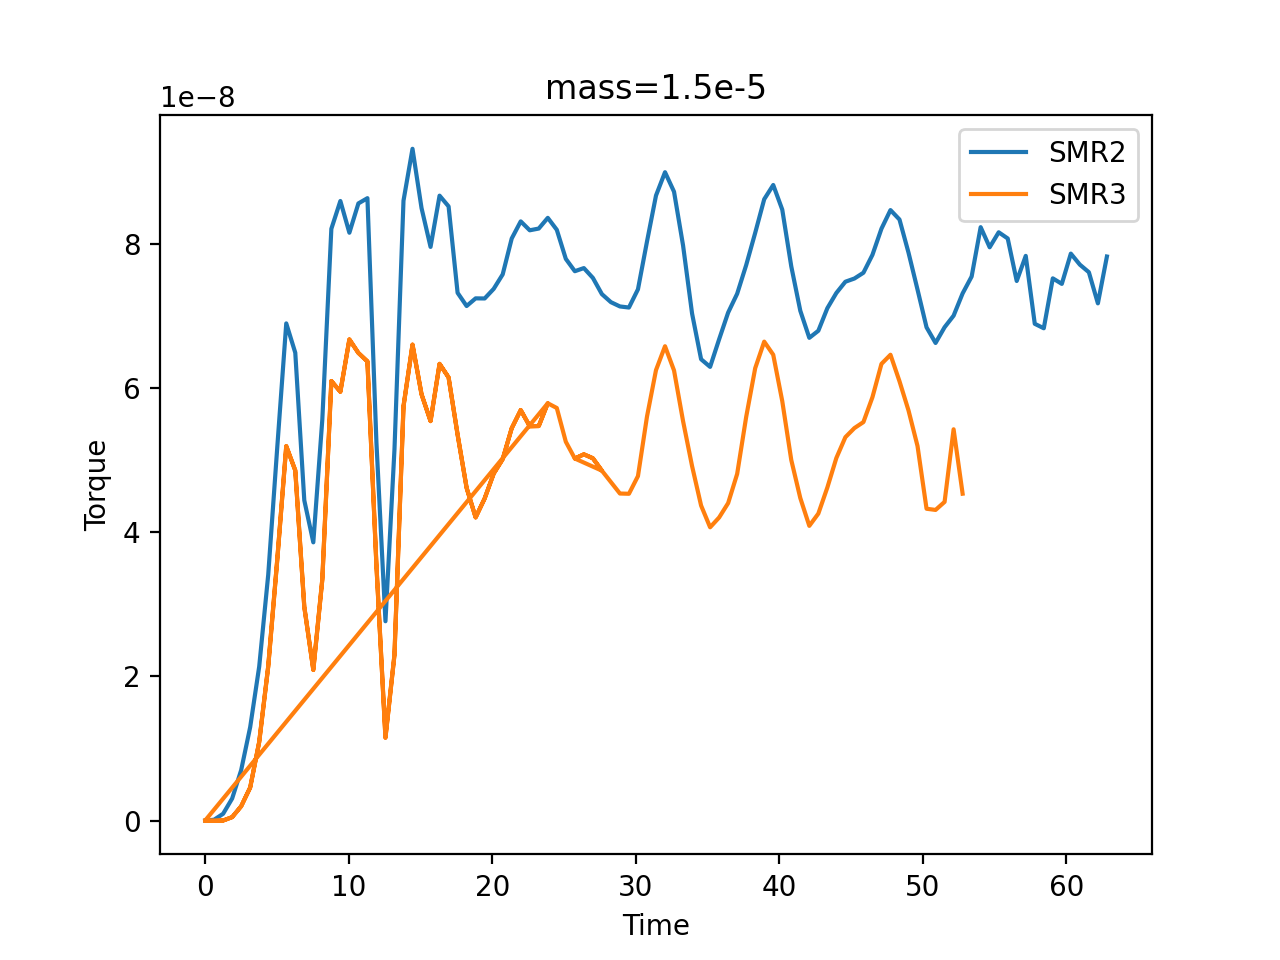
\includegraphics[width=0.6\columnwidth]{comparison_torques.png}
    \caption{The comparison between the torques.}
    \label{fig:twotorques}
\end{figure}



\subsection{Energy injection and transport}
I injected the energy of value $L_c=24\times 10^{-11}$ (times the time) into the sphere of radius $0.003 r_p$ (8 cells) around the planet location.

The thermal diffusivity is $\chi=0.00013 H^2\Omega$ with $\lambda_c=0.5r_p$. The Eq. \ref{eq:diffusivity} is taken from the Eq. 17 in \citet{hankla20}. 
Look at the Figure \ref{fig:den_smr3} to see how the disk looks like with these parameters (including the thermal diffusivity). 
\begin{equation}\label{eq:diffusivity}
    \chi=\frac{3\lambda_c^2\gamma\Omega_0}{8\pi^2}
\end{equation}

\begin{figure}
\centering
	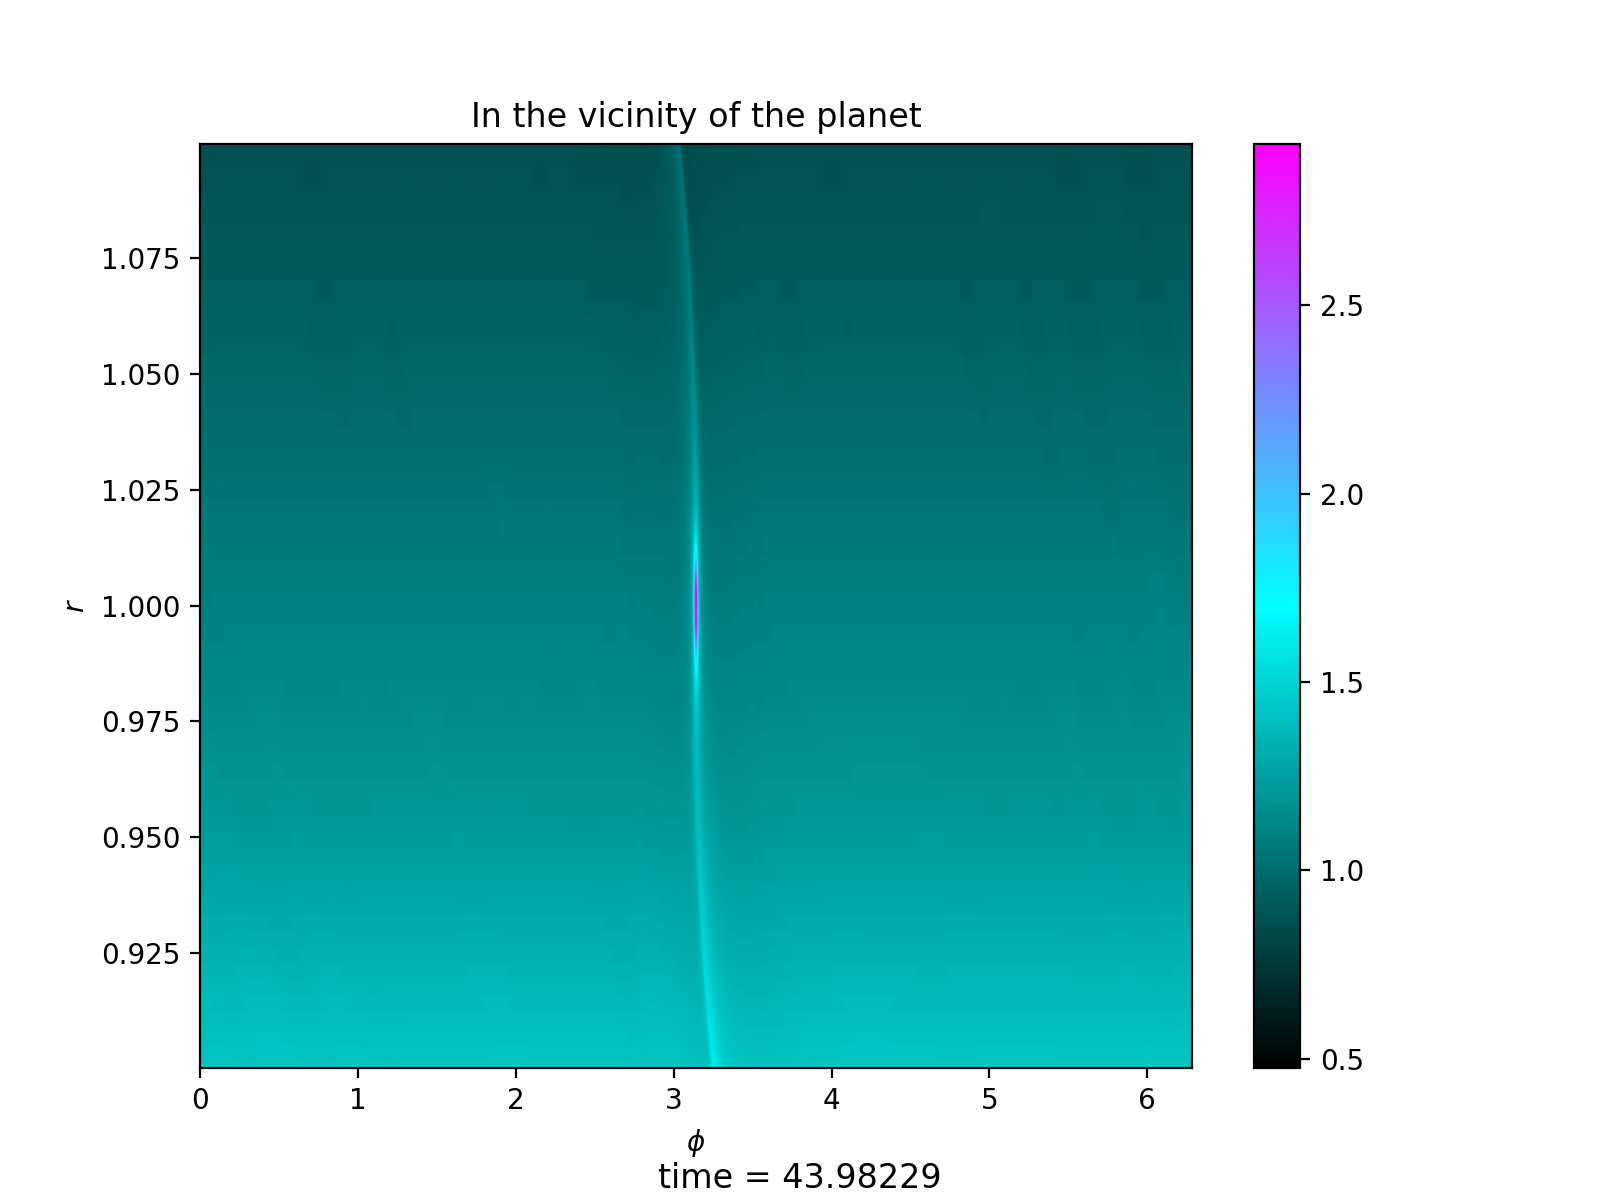
\includegraphics[width=0.48\columnwidth]{smr3zoomeddisk.png}
	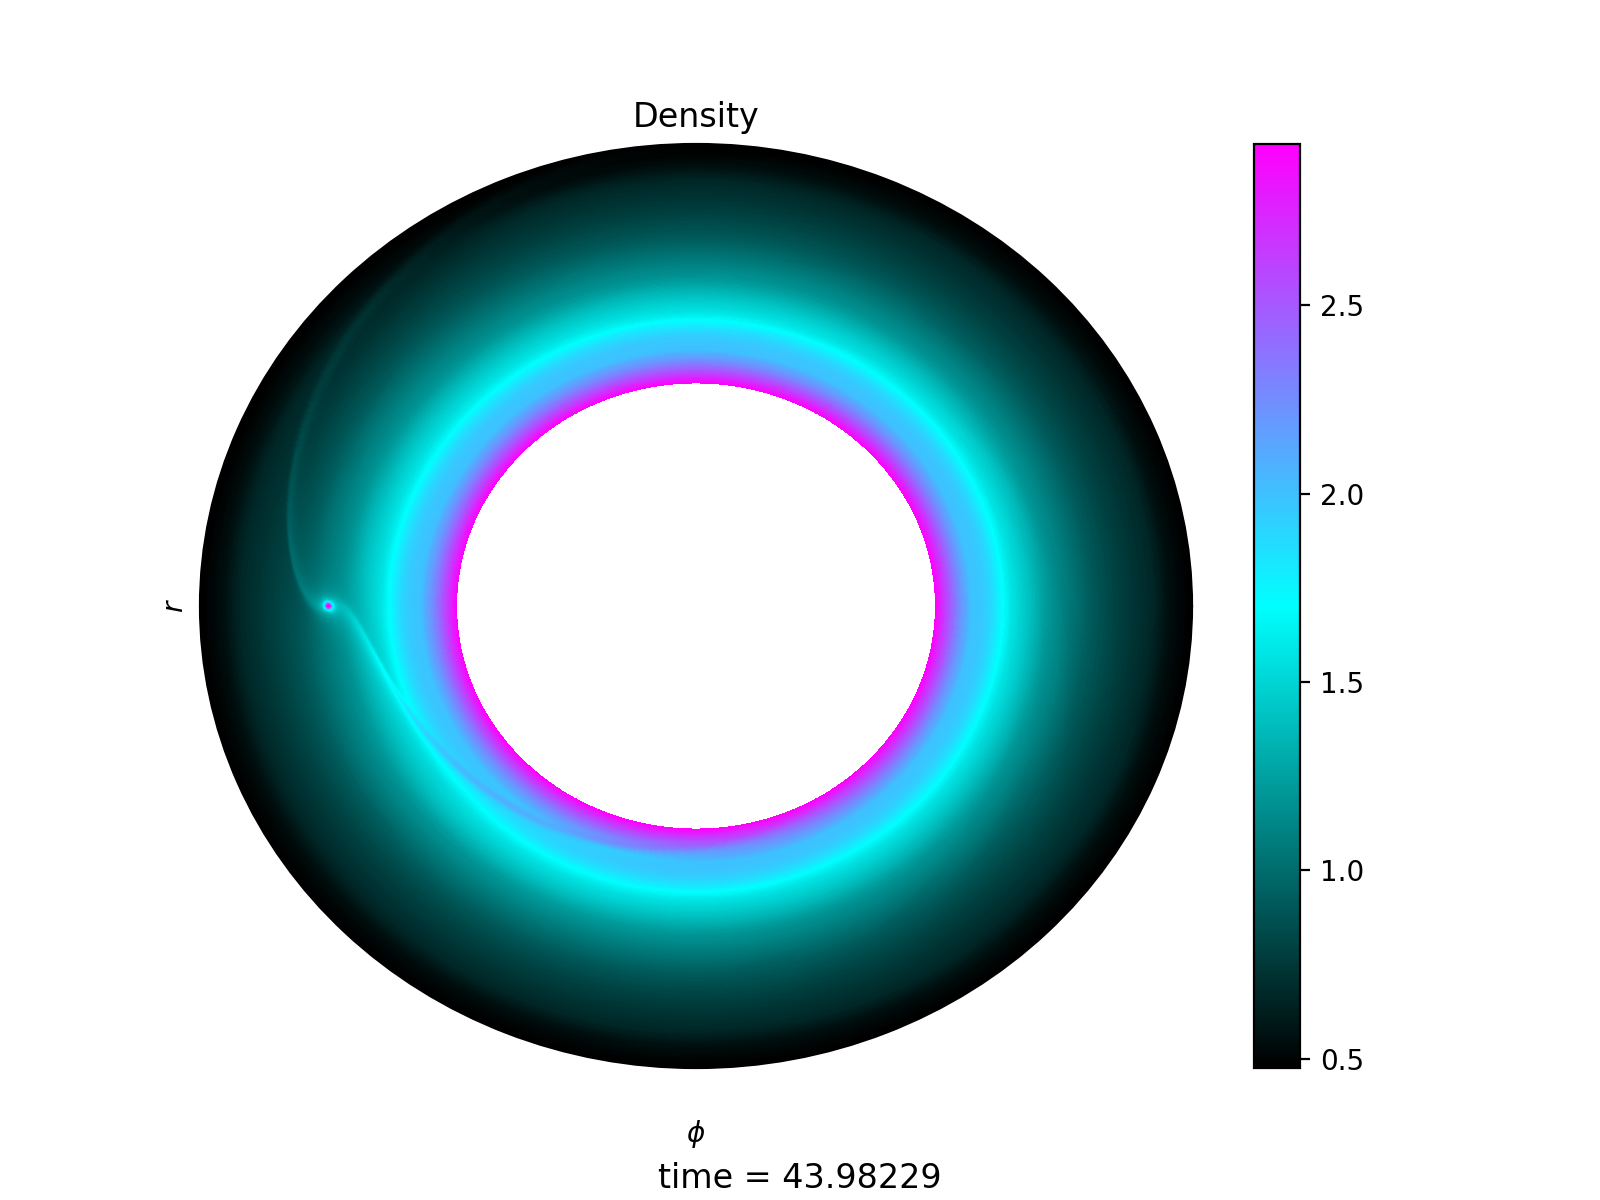
\includegraphics[width=0.48\columnwidth]{smr3disk.png}
    \caption{The density profile of the disk with a perturber with SMR level $l=3$ at the 7th global orbit.}
    \label{fig:den_smr3}
\end{figure}





\subsection{Athena++ simulations}

\section{Results}
\label{sec:results}

\section{Discussion} 
\label{sec:conclusion}

\bibliography{bib}

\end{document}
